\documentclass{article}

\usepackage{amsfonts}
\usepackage{mathtools}
\usepackage{amsthm}
\usepackage{mathrsfs}
\usepackage{amsmath}
\usepackage{graphicx}
\usepackage{hyperref}
\usepackage{stackengine}
\usepackage[mathscr]{eucal}
\usepackage{listings}
\usepackage{algorithm}
\usepackage{algpseudocode}
\usepackage{float}
\usepackage{xcolor}
\usepackage{url}
\newtheorem{theorem}{Theorem}
\theoremstyle{definition}\newtheorem{definition}{DEF}
\theoremstyle{definition}\newtheorem{example}{Ex}
\theoremstyle{lemma}\newtheorem{lemma}{Lemma}
\theoremstyle{corrolary}\newtheorem{corrolary}{Cor}
\setlength{\parindent}{0pt}
\definecolor{codebg}{RGB}{248,248,248}
\definecolor{codekeyword}{RGB}{0,76,153}
\definecolor{codecomment}{RGB}{0,128,96}
\definecolor{codestring}{RGB}{163,21,21}
\definecolor{codenumber}{RGB}{102,102,102}
\lstdefinestyle{pythoncode}{
    language=Python,
    basicstyle=\ttfamily\small,
    keywordstyle=\color{codekeyword}\bfseries,
    commentstyle=\color{codecomment}\itshape,
    stringstyle=\color{codestring},
    numberstyle=\scriptsize\color{codenumber},
    numbers=left,
    numbersep=10pt,
    stepnumber=1,
    showstringspaces=false,
    breaklines=true,
    keepspaces=true,
    columns=fullflexible,
    tabsize=4,
    frame=single,
    framerule=0pt,
    rulecolor=\color{codebg},
    backgroundcolor=\color{codebg}
}
\lstset{style=pythoncode}

\begin{document}

In Part I we discussed the theory of probability, which allows us to characterize the outcome of a random experiment.
The examples we have used so far are simple experiments such as rollling dice and selecting points from a disk.
However, statistics is genrally applied to scientific problems and predicting realowrld outcomes.
As such, we need an understanding of what makes good experimental design and how to connect real-world processes to the outcomes of random experiments.

\begin{definition}
A sample is an element of a sample space.
\end{definition}

\begin{definition}
A population is a set from which a sample space is produced.
\end{definition}

\begin{example}
Consider drawing 2 points from $\mathbb{D}^2$ and computing the distance between them.
In this case, teh population is $P=\mathbb{D}^2$ and the sample space is $S=P^2$.
\end{example}

\begin{definition}
A sampling technique is a transformation that turns a population $P$ and number $n\in \mathbb{N}$ into a probability space $(S, \Omega, p)$.
We say that $n$ is the sample size.
\end{definition}

\begin{definition}
Say a simple random sample (SRS) is a sampling technique that generates a probability space $(S, \Omega, p)$ such ath:
\begin{enumerate}
\item $S$ is the set of all subsets of $P$ of size $n$.
\item $\Omega = \mathcal{P}(S)$
\item $p$ is fair
\end{enumerate}
\end{definition}

\begin{example}
Suppose you have 50 people in a classand you wish to survey a sample 10 of htem to see how they rate the class.
You list everyone in alphabetical order and use MT19937 (Ex \ref{MT19937}) to randomly slect 10 numbers from 1 to 50 without replacement via rejection sampling, then poll hte chosen students.
This is an SRS.
\end{example}

\begin{theorem}
Let $P$ be a population, $f: P\rightarrow \mathbb{R}$, and $(S, \Omega, p)$ be the result of an SRS.
Let $X$ be a random vector such that if $s=(s_1, s_2, ..., s_n)$,  $X(s)=(f(s_1, s_2, ..., s_n)$.
Then the components of $X$ are asymptotically equivalent to iid random variables.
\end{theorem}
\begin{proof}
First, consider the probability space $(P, \mathcal{P}(P), q)$ where $q$ is fair.
Then taking $n$ samples and let $F_k = f(s_k)$ for $1\leq k \leq n$.
Then all $F_k$ are iid random variables.
Additionally, by construction, $F_k$ and $X_k$ have the same distribution. 
Suppose $|P|=\infty$.
Then $\Pr (X_i = X_j | i\neq j)=0$.
Thus, the joint distribution of $X$ and $F$ are the same. \\
Now suppose $|P|=N$.
In this case, the joint distributions of $X$ and $F$ are different because $\Pr (X_i = X_j | i\neq j)\neq 0$ and $\Pr (F_i = F_j | i\neq j)=0$.
Instead, we must show asymptotic convergence as $N \rightarrow \infty$.
Let $U\subseteq \mathbb{R}$ and $\chi_U$ be the indicator function.
Then $\sum_k \chi_U (F_k) \sim Binom(n, \frac{K}{N})$.
Let $|f^{-1}(U)|=K$.
Then $\sum_k \chi_U (X_k) \sim HypGeo(N, n, K)$.
SO $\sum_k \chi_U (F_k) - \sum_k \chi_U (X_k) {D \atop \rightarrow} 0$.
Indeed,
\begin{align*}
f_F(k) - F_X(k)
&= \binom{n}{k} \left(\frac{K}{N}\right)^k \left( 1-\frac{K}{N}\right)^{n-k} - \binom{n}{k}\binom{N-n}{K-k}\binom{N}{K}^{-1}\\
&= \binom{n}{k} \left( \frac{K^k(N-K)^{n-k}}{N^n} - \frac{(N-n)!K!(N-K)!}{(K-k)!(N-n-K+k)!N!}\right) \\
&\rightarrow \binom{n}{k} \left( 
\begin{multlined}
\frac{K^k(N-K)^{n-k}}{N^n} - \\
\frac{(N-n)^{N-n}e^{-(N-n)}K^Ke^{-K}(N-K)^{N-K}e^{-(N-K)}}{(K-k)^{K-k}e^{-(K-k)}(N-n-K+k)^{(N-n-K+k)}e^{-(N-n+K-k)}N^Ne^{-N}}
\end{multlined}
\right) \\
&= \binom{n}{k} \left( 
\frac{K^k(N-K)^{n-k}}{N^n} -
\frac{(N-n)^{N-n}K^K(N-K)^{N-K}}{(K-k)^{K-k}(N-n-K+k)^{(N-n-K+k)}N^N}
\right) \\
&\rightarrow \binom{n}{k} \left( \frac{K^k(N-K)^{n-k}}{N^n} - \frac{K^k (N-K)^{n-k}}{N^n} \right) \\
&=0
\end{align*}
For this first step in convergence we have used Stirling's approximation to replace the factorials.
For the second one, we have leveraged that as $N,K\rightarrow \infty$, $(N-n), (K-k)\rightarrow N,K$.
Thus, we see the convergence in distributions.
Therefore, we have the sample approach iid random variables.
\end{proof}

An SRS is commonly described as a technique in which we sample $n$ items from teh population such that any subset of size $k$ is equally likely to be in the the sample.

\begin{definition}
Let $P$ be a population and $F=\{A_i\}$ be a partition of $P$.
Say $F$ is a factor and $A_i$ is a level of $F$.
\end{definition}

\begin{example}
Suppose we have a bag with 20 marbles, 7 red, 8 blue, and 5 green.
The color is a factor and red, blue and green are levels.
\end{example}

\begin{lemma}
Let $P$ be a population with factor $F$ and levels $\{A_i\}$.
Let $p_i$ be the proportion of elements in $P$ that are in $A_i$.
Let $(S, \Omega, p)$ be the result of an SRS of size $n$.
Then the average number of elements in the SRS with level $i$ is $np_i$.
\end{lemma}
\begin{proof}
First, let $s\in S$ be the sample and let $x\in s$.
Then $\chi_{A_i}(x)$ is a random variable with a Bernouli distribution and probability $p_i$.
If $P$ is infinite, then we have the sum of independent Bernouli variables, which has mean $np_i$.
On the other hand, if $P$ is finite, the result is hypergeometric, which also has mean $np_i$.
So the result holds in either case.
\end{proof}

\begin{definition}
Let $P$ be a population with factor $F=\{A_i\}$ and let $p_i$ be the proportion of objects in level $i$.
Let $S_i, \Omega_i, q_i)$ be the result of an SRS in $A_i$.
Say the product space $(\bigtimes_i S_i, \mathcal{M}(\bigtimes_i \Omega_i ), p)$ is a stratified random sample.
\end{definition}

\begin{example}
Political affiliation can vary a lot by demographic groups, so an SRS can be highly inaccurate.
A better way to sample is to break the population up into demographic groups and poll an SRS of each group to find the outcome.
This data is then combined with the appropriate weighting to predict the election outcome.
\end{example}

\begin{theorem}
Stratified random samples preserve expected value but reduce variance.
\end{theorem}
\begin{proof}
Let $P$ be a population and $F$ a factor.
Let $(S, \Omega, p)$ be an SRS, and $X$ be a random variable.
Because $A_i \subseteq P$, $S_i \subseteq S$ adn $\Omega_i \subseteq \Omega$.
Thus, if $E \in \Omega_i$, $p_i(E)=\frac{p(E)}{p(A_i)}$.
Therefore, we can define a random variable $X_i$ which is the restriction of $X$ on $(S_i, \Omega_i, p_i)$.
Let $f_i$ be the PDF of $X_i$.
Then the result of the stratified random sample is $Y=\sum_i p_i X_i$ and the PD of $X$ is $p_i f_i$.
Thus, $X$ is a mixture model of $X_i$. \\
Now let $\mathbb{E}[X_i]=\mu_i$ and $Var(X_i)=\sigma_i^2$.
Then $\mathbb{E}[X] =\sum_i p_i \mu_i$ by linearity and $\mathbb{E}[Y]=\sum_i p_i \mu_i$ by properties of mixed models (Thm \ref{mixed_model_properties}).
Next, consider that each level's SRS is independent, so we can compute the variance of $Y$ is
\begin{align*}
Var(Y)
&= Var(\sum_i p_i X_i) \\
&= \sum_i p_i Var(X_i) \\
&= \sum_i p_i \sigma_i^2
\end{align*}
By properties of mixed models, $Var(X)=\sum_i p_i \sigma_i^2 + p_i (\mu_i - \mu)^2$.
Clearly, $(\mu_i - \mu)^2\geq 0$, so $Var(X)>Var(Y)$.
Thus, a stratified random sample preserves expected value while reducing variance.
\end{proof}

\begin{definition}
Let $P$ be a population with SRS $(S, \Omega, p)$.
Let $(T, \Phi, q)$ be the result of a different sampling technique.
Let $X: (S, \Omega, p) \rightarrow \mathbb{R}$ and $\tilde{X}: (T, \Phi, q) \rightarrow \mathbb{R}$ be two random variables that represent the same underlying phenomenon.
Say there is sampling bias in the sampling technique if $\mathbb[X] \neq \mathbb{E}[\tilde{X}]$.
\end{definition}

Sampling bias is the idea that the results of a statistical analysis are not representative of the population due to the way the data was collected.
The SRS is the gold standard of sampling techniques because it does not favor any particular subset of hte population.
However there are some drawbacks that can be mitigated with other sampling techniques, such as the reduction of variance with a stratified random sample.
Thus, we need to compare other techniques to the SRS to ensure they do not favor any particular outcomes.

\begin{definition}
A convenience sample is a sampling technique where elements of a population are chosen based on their convenience.
\end{definition}

\begin{example}
A reporter could use a convenience sample to conduct street interviews and ask people's opinions on gun control.
If the reporter is at a gun show then the results would not be representative of hte overall population.
Thus, the sample is biased.
\end{example}

\begin{definition}
Voluntary response bias is a sampling bias is a bias introduced when the sampling technique is whoever wants to volunteer.
\end{definition}

\begin{definition}
Non-response bias is a type of sampling bias in which some of the selected members do not supply the required data.
\end{definition}

\begin{example}
A news station runs a story on a woman who got arrested after putting soda in a water cup at a fast food restaurant.
If the news station asks viewers to call in with their thoughts, the results they get fro mtheir viewers will have voluntary response bias.
On the other hand, if the station takes an SRS of 50 people and only gets responses from 37 they suffer from non-response bias.
\end{example}

When surveying people, the responses are often more likely to be strong negative opinions.
This is very applicable for voluntary response bias, and can also skew results in a non-response bias.
This is why we have to be careful about how we are sampling data.

\begin{definition}
Selection bias is the result of a sampling technique that chooses subjects predisposed to a particular outcome.
\end{definition}

\begin{example}
A survey of outdoor activities is done by taking an SRS of people subscribed to a hiking mailing list.
This is sampling bias, because people who subscribe to a hiking mailing list are more likely to be more interested in outdoor activities.
\end{example}

\begin{definition}
Let $P$ be a population.
Cluster sampling is a technique where $P$ is partitioned into similar subsets and a number of those subsets are chosen at random.
\end{definition}

Cluster sampling is not considered a good sampling technique because there is not enough randomness.
The clusters may seem equivalent, but we can never be sure that they are truly uniform.
Instead, there may be hidden factors that we are unaware of and introduce bias into the results.
On the other hand, stratified random sampling controls levels of a known factor and selects from within each level.
This level of randomness can account for hidden factors that would get captured by an entire cluster.

\begin{definition}
A systemic sample is a sampling technique in which every $k^{th}$ element of a population is sampled.
\end{definition}

\begin{example}
An apartment complex does a survey on noise and they poll every $10^{th}$ apartment.
If the noise is concentrated on one side of the apartment building, you need to sample from both sides for an accurate view, but even numbered apartments are typically on one side of the hallway.
Thus, systemic samplling has a bias.
\end{example}

\begin{definition}
Multistage sampling is a sampling technique in which a population is partitioned into separate groups, some groups are sampled, and then some individuals are sample fro the chosen groups.
\end{definition}

\begin{definition}
Let $P\subset H$.
Rejection sampling is a technique in which individuals are sampled from $H$ and then removed if they are in $H\backslash P$ and new individuals are sampled to replace them.
\end{definition}

Recall we have discussed rejection sampling in example \ref{circle_rejection_sampling}.

\begin{example}
In order to predict election outcomes, we want to survey likely voters.
One way to do this is to select people in the area and determine whether they are likely to vote, then reject htose that are not and sample more.
This is an application of rejection sampling.
\end{example}

\begin{definition}
A poll is when people are asked a question.
\end{definition}

\begin{definition}
A census is when an entire population is polled.
\end{definition}

\begin{definition}
A survey is when a sample of individuals is polled.
\end{definition}

In general, it is ideal to take a census to get all hte info about a population.
However, this is often impossible due to either logisitcal reasons or physical impossibility.
For example, it would be too expensive to ask every American how they would vote in an upcoming election.
Thus, we will usually take a survey that is representative of the population and generalize to draw conclusions about hte entire population.

\begin{definition}
An experiment is a study in which a treatment is imposed.
\end{definition}

\begin{example}
A study is performed to determine the effectiveness of seat belts.
In order to do so, crash test dummies are put into cars, some of which have seatbelts and others do not, and the cars are crashed into each other.
This is an experiment, as the researchers determine which dummies do and do not have seatbelts.
\end{example}

\begin{definition}
An observational study is a study in which treatments are not imposed.
\end{definition}

\begin{example}
A study is performed to determine the effectiveness of seat belts.
Researchers look through records of past crashes to determine the fatality and severity of injuries and whether or not the victims were wearing seat belts.
Then the crash results are compared for the two groups to determine whether seat belts are helpful in crashes.
This is an observational study as the researchers are not determining who does and does not wear a seatbelt.
\end{example}

Generally, experiments are better at for determining results.
However, experiments may not always be possible or ethical to perform, so observational studies are also helpful.
For example, it would be unethical to crash people in cars intentionally, so we can either look at historical data or use dummies to get data.

\begin{definition}
A subject is a person or object on which an expirement is performed.
\end{definition}

\begin{definition}
A placebo is a dummy treatment.
\end{definition}

\begin{definition}
The placebo effect is when any treatment, even a dummy treatment, has an effect.
\end{definition}

\begin{example}
Stomach ulcers cause heat in the stomach, so an initial tratment idea was to put cold air in a patient's stomach.
Initial studies found that this treatment could reduce ulcers by up to 80\%.
However, an expirement was performed to compare cold air against a placebo and the 80\% reduction was the same.
Now, placebos are a common treatment for stomach ulcers.
\end{example}

\begin{definition}
Control is when researchers tke steps to account for the effects of an outside variable on the results of an experiment.
\end{definition}

\begin{definition}
A control group is an expiremental group that receives a placeb oin order to increase control.
\end{definition}

\begin{example}
An expirement is performed to see the effects of a new fertilizer on crop yield.
A 60 acre plot of land is divided into one acre portions, some of which are sunny and some of which are shady, and a stratified random sample is taken to split the portions into 3 partitions.
One group receives the new fertilizer, one group receives an existing fertilizer, and one group receives no fertilizer.
THe stratified random sample is an example of control to account for differences in sunlight on crop yield.
THe group that receives no fertilizer is a control group for the experiment because they receive no treatment.
We are interested in seeing if hte new fertilizer outperforms the old one, but the old one is a treatment, so that group is not considered a control group.
\end{example}

\begin{definition}
Replication is the prectice of using more samples per treatment in order to better represent the population.
\end{definition}

\begin{example}
In the fertilizer experiment, it is better to have 20 one acre patches per treatment than 15 one acre patches per treatment.
\end{example}

\begin{definition}
Randomization is when treatments are assigned to subjects in a randomized (i.e. probabalistic) manner.
\end{definition}

\begin{example}
Assigning the fertilizer treatments to the plots via a stratified random sample is an element of randomness in the experiment.
\end{example}

\begin{definition}
A well designed experiment is one that includes randomization, replication, and control 
\end{definition}

\begin{definition}
A completely randomized design (CRD) is a randomization technique in which a random permutation of the subjects is chosen uniformly and the experimental groups are based on the permutation.
\end{definition}

\begin{theorem}
A CRD is equivalent to an SRS
\end{theorem}
\begin{proof}
Let there be $n$ subjects and let $\alpha$ be a permutation of $\{1, 2, ..., n\}$.
Suppose we have $k<n$ subjects in experimental group 1.
THen by definition of CRD, the subjects in group 1 are $\{\alpha (1), \alpha(2), ..., \alpha (k)\}$.
For a permuttaion $\beta$, the exerimental groups induced by $\alpha$ and $\beta$ are the same if for all $1\leq i \leq k$ there is some $1 \leq j \leq k$ such that $\alpha (i) = \beta(j)$.
In other words, teh groups are the same if $\beta (1), \beta (2), ..., \beta (k)\}$ is a permutation of $\{\alpha (1), \alpha(2), ..., \alpha (k)\{$.
There are $k! (n-k)!$ such permutations and $n!$ permutations total, so there are $\binom{n}{k}$ possible experimental groups, each of which is equally likely.
Now consider taking an SRS of $k$ items from a population of size $n$.
By construction, we have a fair distribution on all $k$ sized subsets of the population.
Thus, the two are equivalent.
\end{proof}

\begin{definition}
A block design is a randomization strategy in which the subjects are partitioned and a CRD is performed within each partition class.
\end{definition}

\begin{theorem}
A block design is equivalent to a stratified random sample
\end{theorem}
\begin{proof}
Partition the subjects into subsets and call this a factor $F$ with levels $A_i$.
For a block design, we take a CRD in each level $A_i$, which is equivalen to taking an SRS within each $A_i$.
Thus, it is clear that this is equivalent to a stratified random sample.
\end{proof}

\begin{example}
A trial for a new drug has 40 participants, 15 men and 25 women.
A sample of 7 men and 12 women are selected to receive the drug while hte other 8 men and 13 women receive a placebo.
\end{example}

\begin{definition}
Causation is a situation in which a random variable $X$ determines the value of another variable $Y$.
\end{definition}

\begin{center}
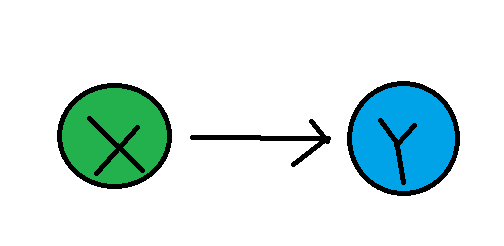
\includegraphics[scale=0.5]{images/causation.png}
\end{center}

\begin{definition}
Common response is a situationi in which an unmeasured random variable $Z$ determines the value of both $X$ and $Y$.
\end{definition}

\begin{center}
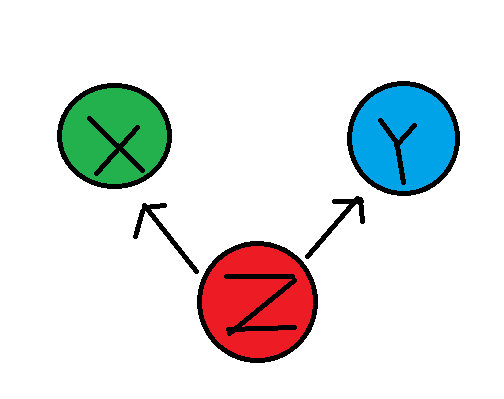
\includegraphics[scale=0.5]{images/common_response.png}
\end{center}

\begin{definition}
Confounding response is a situation in which a random variable $X$ and an unmeasured random variable $Z$ together determine the value of a variable $Y$.
In this case, we say $Z$ is a confounding variable.
\end{definition}

\begin{center}
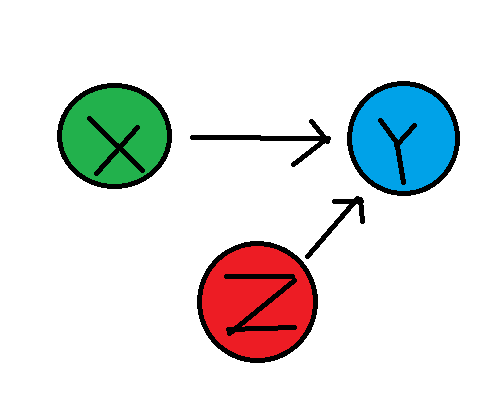
\includegraphics[scale=0.5]{images/confounding_response.png}
\end{center}

It is often said that correlcation does not imply causation.
In all three types of relationships described there is (or at least can be) correlation between $X$ and $Y$, but only one of them is a causation relationship.

\begin{example}
Shark attacks are highly correlated with ice cream sales.
This is an example of common response, as both are caused by temperature.
When it is hot out, people buy more ice cream and go to the beach more, which increases shark attacks.
The relationship between temperature and ice cream sales would be an example of causation.
\end{example}

\begin{example}
The relationship between smoking nad cancer is a confounding response.
Smoking does cause cancer, but genetics is a confounding variable that drives cancer.
\end{example}

Only a well designed experiment can show causation.
The goal of control is to prevent a confounding variable from indicating a causal relationship that does not exist.
Both experimental groups have similar amounts of the confounding variable, so it will not drive a noticeable effect.
The issue with this approach is that there can always be more confounding variables that we either can not control or simply did not consider.
As such, the randomness ensures that on average it will be consistent across the experimental groups.
With a small sample size, we may see large differences in confounding variables just by chance, but larger sample sizes reduce this variability.
This is why randomness and replication are important in an experiment.

\end{document}
